\section{QCD Background Estimation Methods}

\label{sec:QCD_bkgd_est}

In the context of a search for SUSY using a signature containing an electron, there are three sources of ``background electrons'', namely ``non-prompt'' electrons:
\begin{enumerate}
\item Jets which are either mismeasured or have very atypical hadronization, yielding ``electrons'' which pass the basic identification and selection requirements.  We refer to these as ``Jet electrons'' (Jet-e) in what follows.
\item Photon conversions in the tracker material.  We refer to these as ``Conversion electrons'' (Conv-e) in what follows.
\item Electrons from semileptonic decays of $c$ and $b-$ flavored hadrons.  We refer to these as ``Heavy Flavor electrons'' (HF-e) in what follows.
\end{enumerate}

There are numerous methods for estimating both the amount of background remaining in a data sample after a specific set of selection cuts and the shape of this background as a function of various variables (the transverse momentum, pseudorapidity, and in some cases more complicated topological variables).  All these methods employ ``control samples'' which are selected via appropriate alternate requirements which do not affect the shape of the variable in question (e.g. the transverse momentum of the lepton).  As an example, we mention the well-known ``Isolation inversion'' method, where one uses events failing the isolation requirement and an extrapolation into the ``selection region'', i.e. where events pass the isolation requirement, to estimate the amount of background in the latter[GEORGIA: REF to Cornell].  A crucial issue in most methods is the demonstration that the extrapolation from the ``control region'' to the ``selection region'' is correct or, at least, its deficiencies are small and can be estimated reliably.  There are two elements that enter this extrapolation from a control region to a selection region in the case of electrons:
\begin{itemize}
\item The actual knowledge of the full dependence of any single source of background electrons on the variable in question.  As an example, concentrating on only the Jet-e background, there remains the issue of how to obtain reliably the full shape of the isolation of the Jet-e background which passes all selection cuts from some other ``control sample'' which passes a slightly different set of cuts.
\item The presence of the three different sources of background implies that each of these backgrounds may well exhibit a different dependence on the variable in question.  As an example, the isolation distribution from Jet-e and Conv-e need not be (and is in fact not) the same.  This implies that it may be necessary to determine explicitly the amount of each background in the selection region, and to then form the total expected background as the sum of the three individual components.
\end{itemize}
For the sake of concreteness, in what follows we will refer to the ``Isolation variable'', even though the discussion applies equally well to essentially most variables.

Of the two above issues, the first is usually tackled initially using Monte Carlo: one uses generator-level information to obtain the Isolation distribution for any specific background (e.g. Jet-e) and then compares this shape with that extracted from the ``control sample''.  Assuming that this comparison is favorable, i.e. that the shape from the control sample can adequately describe the shape in the selection sample, the next and final step is to compare this shape with the one extracted from data using the ``control selection''. 

Tackling the second issue is more complicated though. First, the presence of three sources of background (instead of two) implies more degrees of freedom in the fitting (and in general in describing) any particular variable -- e.g. the Isolation variable. Second, the relative amount of each source needs to be determined for the final selection sample.

In this section, we concentrate on the following three key observations to address all of the above:
\begin{enumerate}
\item A good method for identifying a control sample for the Jet-e background is the reversal of the matching cuts $\Delta\eta$ and $\Delta\phi$.  These two variables exhibit near independence from other selection variables, especially the isolation variable
\item The isolation distributions of the Jet-e and HF-e backgrounds seem to be similar and to be collectively described well by the same control sample (via the matching-cut reversal).
\item A fairly pure sample of Conv-e background can be identified using the existing conversion-identification tools. This sample can then be used to extract a template for other variables in question, e.g. the Isolation distribution or the $\alpha_T$ distribution.
\end{enumerate}
In what follows, we exploit these three observations to obtain the shapes of the total background in both the isolation and $\alpha_T$ distributions.  Moreover, a fit to the isolation distribution using different shapes (templates) for the Jet-e and Conv-e backgrounds yields an estimate of the absolute number of background events in the selection region.

\subsection{The three electron backgrounds}

In what follows, we will consider more closely two different definitions of ``Isolation'', namely ``Calo Isolation'', which is defined using only the sum of the energies in the ECAL and HCAL, and ``Combined Isolation'' which includes also the transverse momenta of charged-particles tracks around the electron.  Since the search for SUSY may necessitate using low-$P_T$ leptons, we investigate the behavior for two different thresholds of 10 and 20 GeV on the electron $P_T$.

The isolation distribution using only calorimeter isolation is displayed in Figure~\ref{fig:caloIso_MC}, whereas the combined (reltive) isolation is shown in Figure~\ref{fig:combIso_MC}.  It can be seen that two backgrounds, namely the Jet-e and JF-e have distributions which are fairly similar for both the Calo-Iso and Comb-Iso.
\begin{figure}[htb!]
\centering
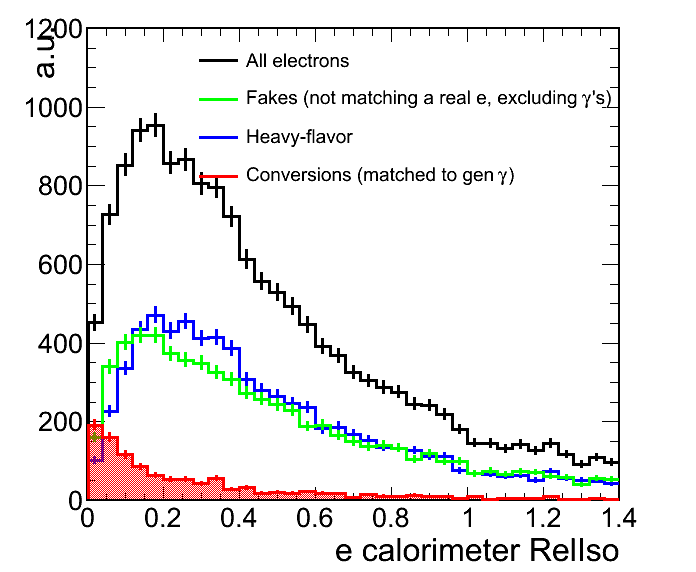
\includegraphics[scale=0.28]{Plots/caloIso_pt10_MC.png}
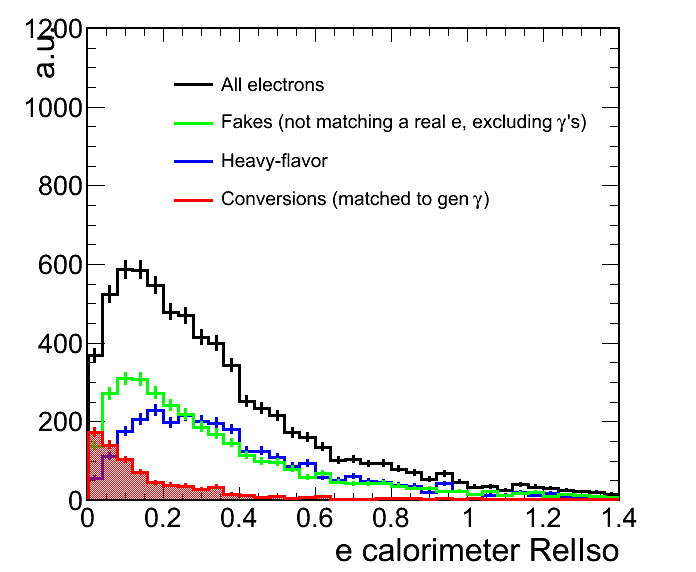
\includegraphics[scale=0.28]{Plots/caloIso_pt20_MC.png}
\caption{The Calorimeter Isolation distribution from Monte Carlo simulation.  On the left for a threshold of 10 GeV on the electron and the right for a 20 GeV threshold.  The three sources of background, name Jet-e, HF-e and Conv-e are shown separately, along with the sum of the three.}\label{fig:caloIso_MC}
\end{figure}

\begin{figure}[h!]
\centering
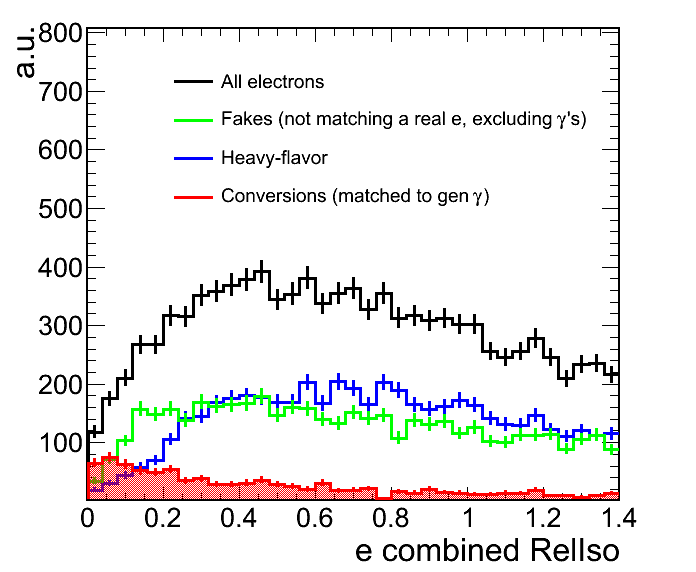
\includegraphics[scale=0.28]{Plots/combIso_pt10_MC.png}
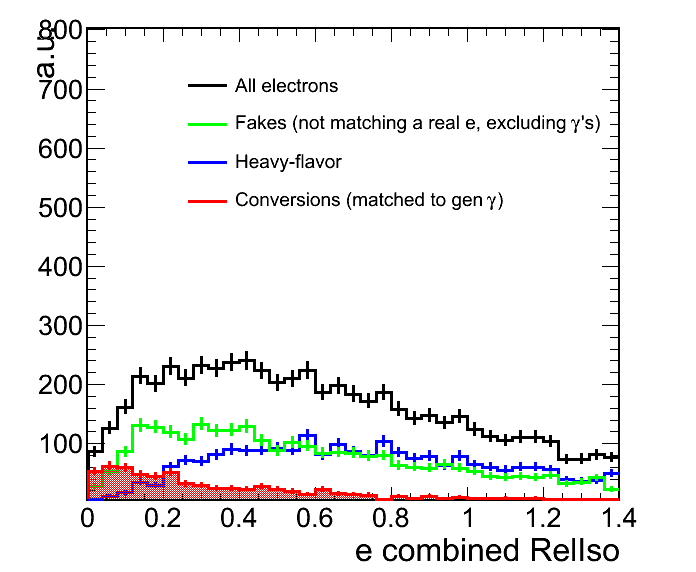
\includegraphics[scale=0.28]{Plots/combIso_pt20_MC.png}
\caption{The Combined Isolation distribution from Monte Carlo simulation.  On the left for a threshold of 10 GeV on the electron and the right for a 20 GeV threshold.  The three sources of background, name Jet-e, HF-e and Conv-e are shown separately, along with the sum of the three.}\label{fig:combIso_MC}
\end{figure}

\subsubsection{Isolation Distribution for the Jet-e and HF-e backgrounds}

The first step is now to define a control sample for the combination of Jet-e and HF-e and to see how well it can describe the Isolation distributions (both CaloIso and CombIso) in the selection region.  As stated previously, this is done by inverting the $\Delta \eta$(trk-SC) and $\Delta \phi$ (trk-SC) id cuts in the electron selection. The selected events in this method pass the pre-selection described in Section~\ref{sec:Sel}, while the anti-selected are those events which pass the selection with an electron that passes all selection id criteria except the $\Delta \phi$ (trk-SC) and $\Delta \eta$(trk-SC) ones.  The resulting distributions are shown in Figure~\ref{fig:caloIso_fakes} for the CaloIso and in Figure~\ref{fig:combIso_fakes} for the CombIso.

\begin{figure}[h!]
\centering
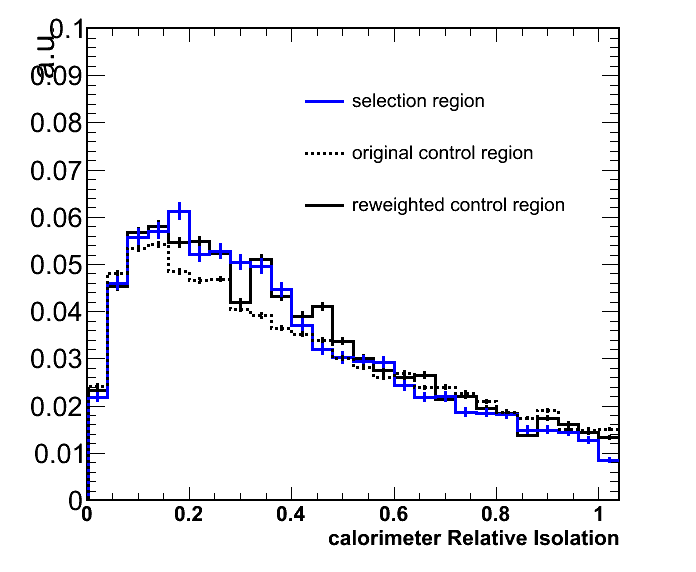
\includegraphics[scale=0.28]{Plots/caloIso_pt10_fakes.png}
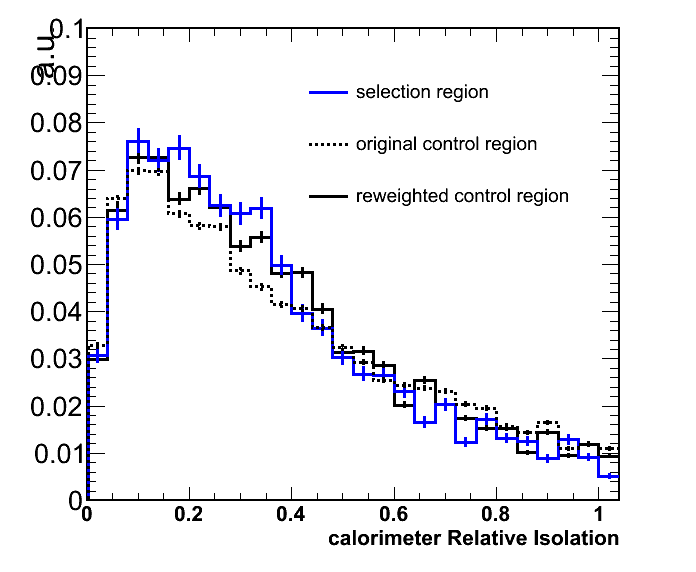
\includegraphics[scale=0.28]{Plots/caloIso_pt20_fakes.png}
\caption{The Calorimeter Isolation distribution from Monte Carlo simulation of the combined Jet-e+HF-e background.   On the left for a threshold of 10 GeV on the electron and the right for a 20 GeV threshold.  The solid blue line is the total Jet-e+HF-e background in the selection region, whereas the dashed line is the distribution from the control sample, defined via the anti-selection on the matching cuts.  The solid black line is the result of re-weighting the control sample for the jet spectra -- as described in the text.}\label{fig:caloIso_fakes}
\end{figure}

\begin{figure}[h!]
\centering
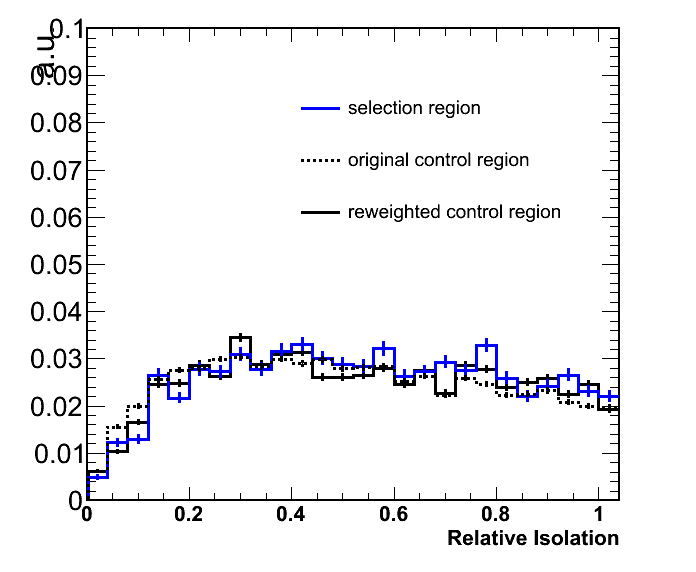
\includegraphics[scale=0.28]{Plots/combIso_pt10_fakes.png}
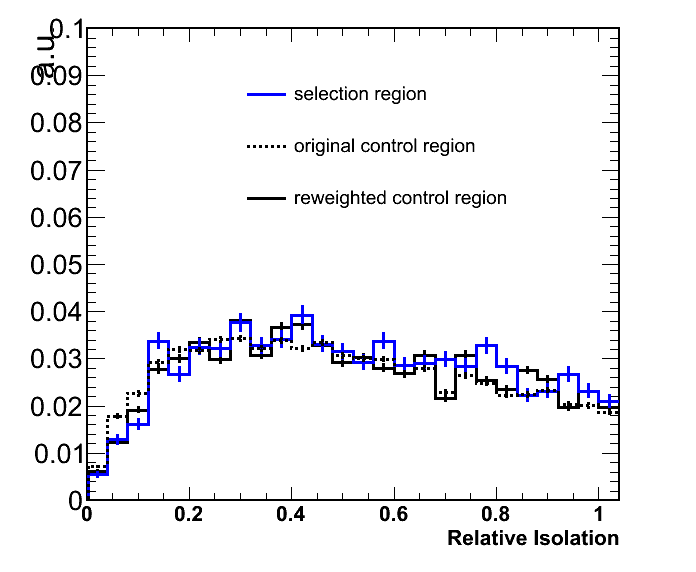
\includegraphics[scale=0.28]{Plots/combIso_pt20_fakes.png}
\caption{Same as Figure~\ref{fig:caloIso_fakes} only this time for the Combined Isolation distribution.}\label{fig:combIso_fakes}
\end{figure}

It can be seen that the shape of the Combined Isolation distribution from the Control Region is very similar to that of the distribution from the Selection Region -- a very encouraging result which indicates that the anti-selection of the matching cuts yields a good method for modeling non-conversion electrons. A closer look into various properties of these events, however, yields a slight difference in the Calorimeter Isolation distributions.  As can be seen in Figure~\ref{fig:caloIso_fakes}, for small values of the CaloIso variable the two distributions, i.e. from the Control and Selection regions have a small difference (around CaloIso$\approx 0.1-0.4$).  This is more easily seen in Figure XYZ where the ratio of the Calorimeter Isolation distributions from the Selection and Control regions is displayed. 

We have investigated possible sources of this difference, from the surrounding objects, and in particular any jet that (possibly) accompanies the electron candidate.  There are small differences in the shapes of the associated jet $P_T$ spectrum as well as from the distance in $\eta-\phi$ space between the jet and the electron.  Presumably, these differences arise from a small correlation between the matching variables and the density of the overall hadronic energy surrounding or near the electron candidate.  Since the difference is small, we have attempted to correct the correct the ``predicted'' shape, i.e. the shape from the Control Region, by applying a weight which depends on the associated Jet $P_T$ and the $\Delta R$ between the jet and the electron.  The solid blue line in \ref{fig:caloIso_fakes} is the result of this re-weighting.  It can be seen that the corrected Calorimeter Isolation distribution from the Control Region now describes the distribution from the Selection Region very well.  We have also applied the same correction to the Combined Isolation distribution, which did not exhibit a visible difference between the Control and Selection Regions, to ensure that the correction did not adversely affect this original agreement.  As can be seen in Figure~\ref{fig:combIso_fakes} the corrected distribution still describes the Selection Region very well.

\subsubsection{Isolation distribution from the Conv-e background}

Electrons from photon conversions are identified using the standard criteria of the Conversion Finder tools \cite{conv}. A suitable Control sample for modeling the Conv-e component in the Isolation distribution can be obtained by electrons that pass the Conversion tools (i.e. using an anti-veto on the Conversion rejection requirements). There are two algorithms to identify electrons from converted photons:

\begin{itemize} 
\item \textit{Missing expected hits}: the algorithm asks that there be $> 0$ expected layers with a missing hit before the first valid hit on the electron's track. The number of missing expected hits in front of the innermost valid hit is available via the electron's gsfTrack Hit Pattern.
\item \textit{Partner track finding}: the algorithm looks for the electron's partner track from a converted photon in the generalTrack collection. The track is identified as a conversion partner if: 
\begin{itemize}
\item the track has opposite charge to the electron track.
\item Approximately the same $\delta \cot(\theta)$ , in this case: $|\delta \cot(\theta)| < 0.02$.
\item small distance (dist) in the $r-\phi$ plane, in this case: $|\text{dist}| < 0.02$. 
\end{itemize}
\end{itemize}

The Conv-e component of the Isolation in the Selection region is formed using only electrons that found a match with a generated photon at MC truth level. The shape of this component is compared with the one obtained from the Conv-e control region as described previously.  

%GEORGIA: please fill in the text describing the algorithm and cuts.

The resulting distributions are shown in Figure~\ref{fig:caloIso_conv} for the CaloIso and in Figure~\ref{fig:combIso_conv} for the CombIso.  It can be seen that the shape of both distributions in the Selection Region is described well by the Control Region.

\begin{figure}[h!]
\centering
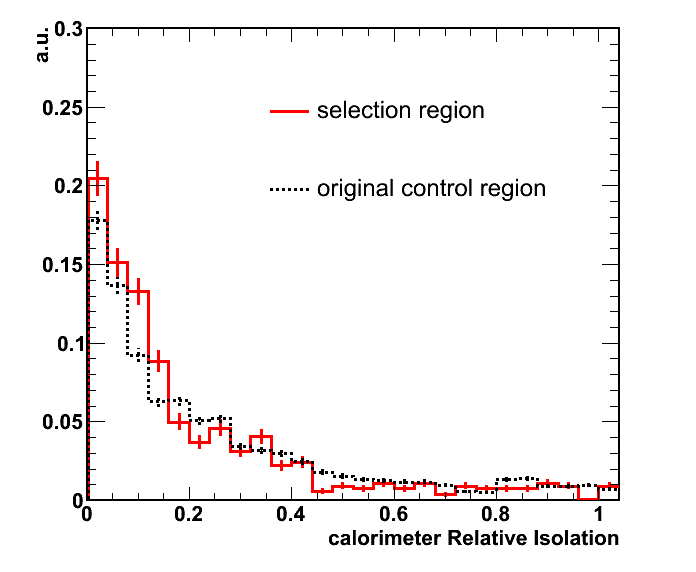
\includegraphics[scale=0.28]{Plots/caloIso_pt10_conv.png}
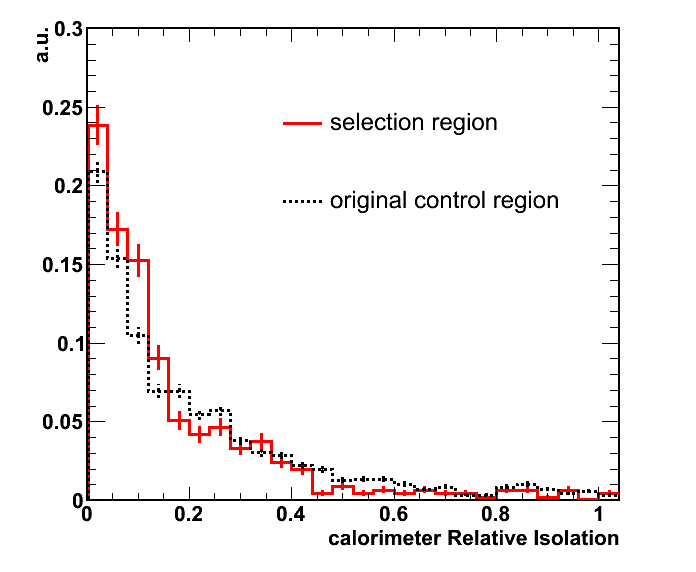
\includegraphics[scale=0.28]{Plots/caloIso_pt20_conv.png}
\caption{The Calorimeter Isolation distribution from Monte Carlo simulation of electrons from conversions.   On the left for a threshold of 10 GeV on the electron and the right for a 20 GeV threshold.  The solid red line is the Conv-e background in the selection region, whereas the dashed line is the distribution from the control sample, defined via the conversion identification requirements described in the text.}\label{fig:caloIso_conv}
\end{figure}

\begin{figure}[h!]
\centering
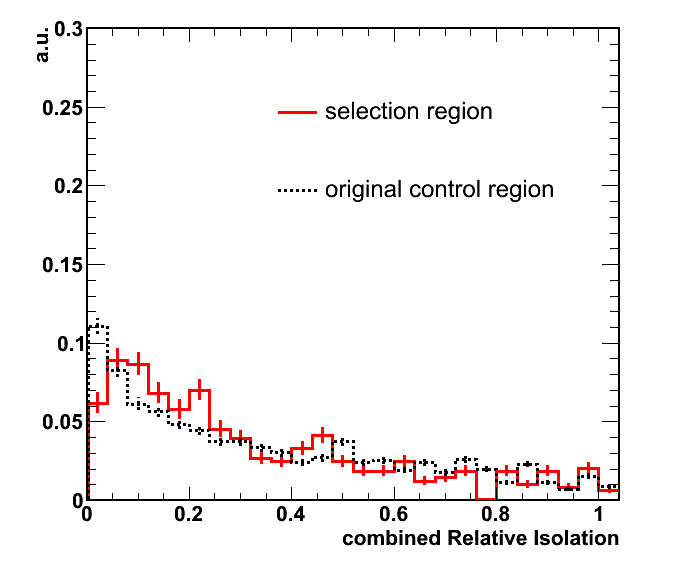
\includegraphics[scale=0.28]{Plots/combIso_pt10_conv.png}
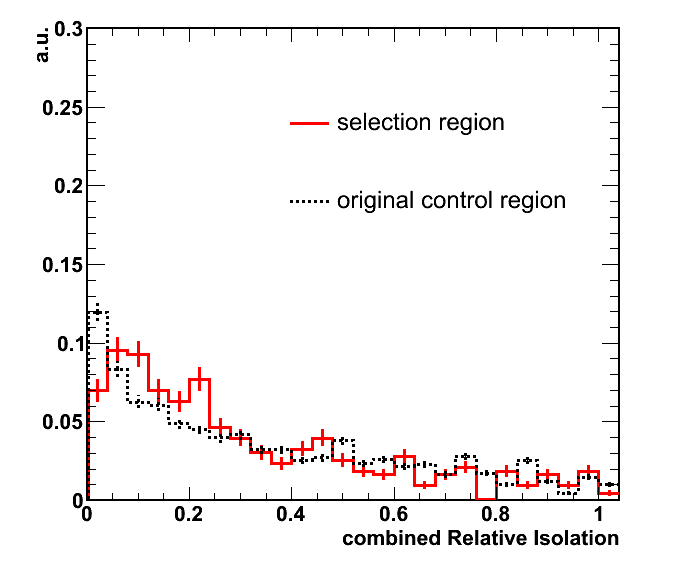
\includegraphics[scale=0.28]{Plots/combIso_pt20_conv.png}
\caption{Same as Figure~\ref{fig:caloIso_conv} only this time for the Combined Isolation distribution.}\label{fig:combIso_conv}
\end{figure}

\subsubsection{Describing the Isolation Distribution in the Selection Region}

Having demonstrated that two independent Control Samples can yield good descriptions of the Isolation distribution in the Selection Region for each background (i.e the combined Jet-e+HF-e and the Conv-e) we next attempt to describe the full Isolation distribution in the Selection Region as a sum of two components, with the template of each component extracted as described above: the combined Jet-e and HF-e background is described from the corrected (re-weighted) anti-selected (for matching) sample, whereas the Conv-e background is described from the sample passing the conversion-identification criteria.  We thus fit the total Isolation distribution using these two components, leaving the relative normalization of the two as a free fit parameter.  The result is shown in Figure~\ref{fig:caloIso_fit} for the calorimeter isolation and shows a very good description of the total background distribution.  It can also be observed that the conversion component becomes more relevant at high $P_T(e)$.  The corresponding distributions for the Combined Isolation variable are described equally well.  In the interest of saving space, and since previously it is the Calorimeter Isolation distribution which exhibited some differences, in what follows we will concentrate only on the Calorimeter Isolation (even though the corresponding Combined Isolation was always checked and found to be in excellent agreement).

\begin{figure}[h!]
\centering
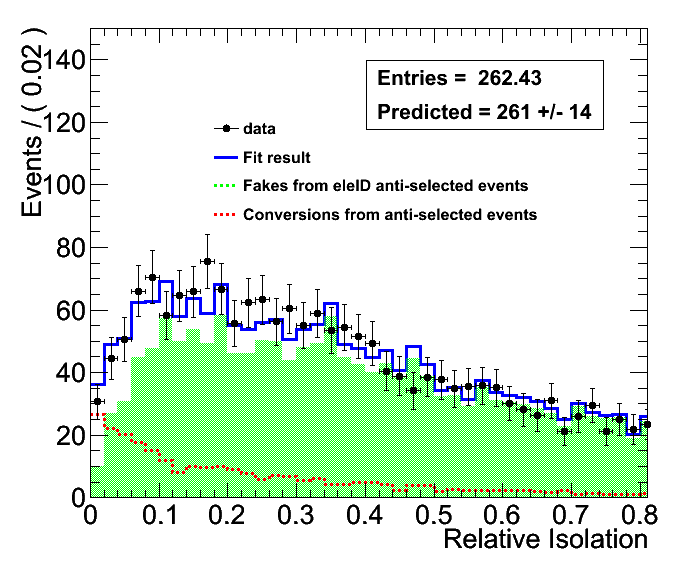
\includegraphics[scale=0.28]{Plots/caloIso_pt10_fit.png}
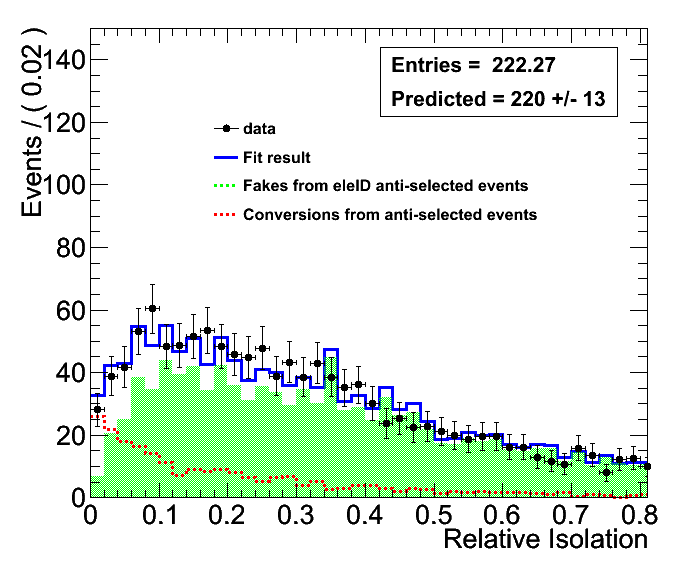
\includegraphics[scale=0.28]{Plots/caloIso_pt20_fit.png}
\caption{The Calorimeter Isolation distribution from Monte Carlo simulation of background electrons. On the left for a threshold of 10 GeV on the electron and the right for a 20 GeV threshold.  The dashed lines are the two background components as extracted from the two Control Samples, whereas the sum of the ``predicted'' background is the solid line.}\label{fig:caloIso_fit}
\end{figure}

Given the remarkably good description of the combined background in Monte Carlo simulation, we next test this procedure on CMS data.  This is the subject of the next section.

\subsubsection{Isolation distribution in 7 TeV data}

The data are selected as in

GEORGIA: please fill in.

Since, as was shown in the previous section, we observed a small deviation between the Calorimeter Isolation distributions in the Control and Selection Regions (prior to re-weighting as described above) we would like to confirm that the good description of the full Isolation distribution, i.e. with all backgrounds combined, remains good for different regions in the overall hadronic selection of the events.  For this region, we repeat the fits for different values of the total HT of the event.  These fits are shown in Figure~\ref{fig:caloIso_fit_HT} for three different cuts on HT (20, 40 and 60 GeV respectively).  It can be seen that the overall description remains very good.  

\begin{figure}[ht]
\centering
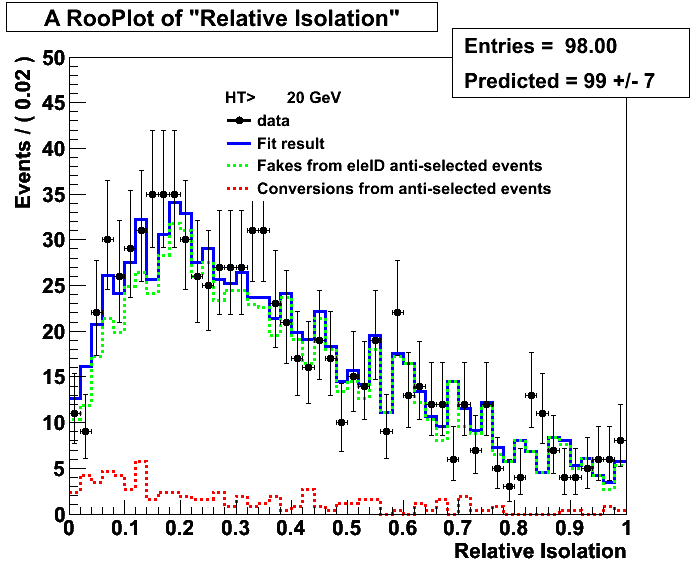
\includegraphics[scale=0.28]{Plots/caloIso_pt10_ht20.png}
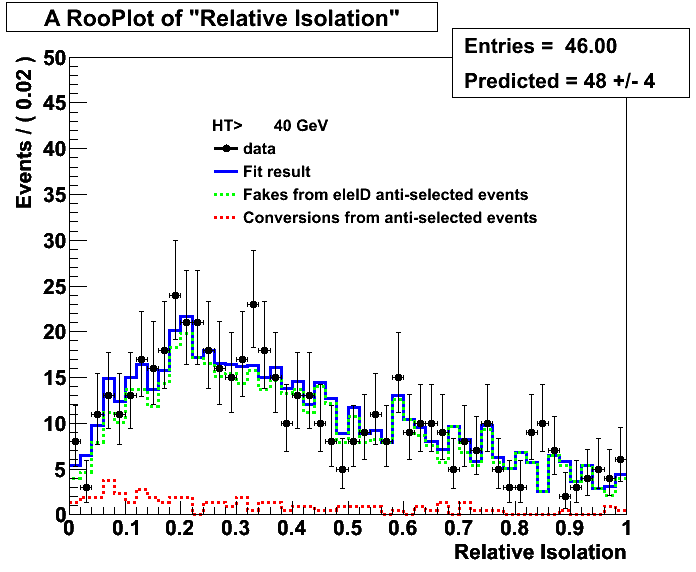
\includegraphics[scale=0.28]{Plots/caloIso_pt10_ht40.png}
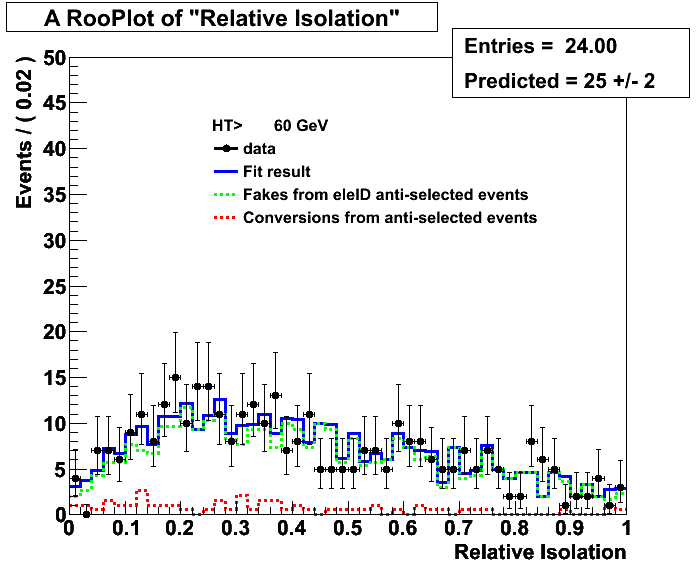
\includegraphics[scale=0.28]{Plots/caloIso_pt10_ht60.png}
\caption{The Calorimeter Isolation distribution in data (points) and its breakdown into two components, one for the combined background from jets and heavy flavors (Jet-e+HF-e) and conversions (Conv-e).  The shapes of the two backgrounds comes from the Control Regions described in the text.  The three figures correspond to three different values (20, 40 and 60 GeV) of the HT cut.}\label{fig:caloIso_fit_HT}
\end{figure}

We have also investigated this agreement for even lower $P_T(e)$ values, in particular for $P_T(e)>5$ GeV.  This is shown in Figure~\ref{fig:caloIso_fit_HT}.  

\begin{figure}[h!]
\centering
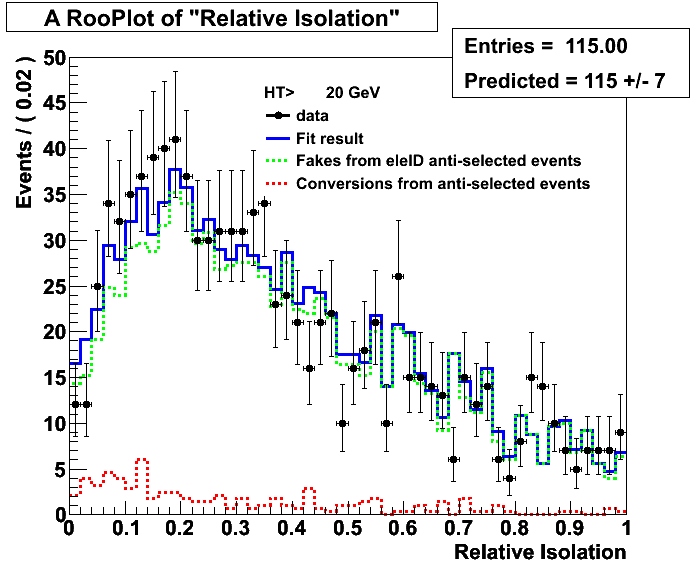
\includegraphics[scale=0.28]{Plots/caloIso_pt5_ht20.png}
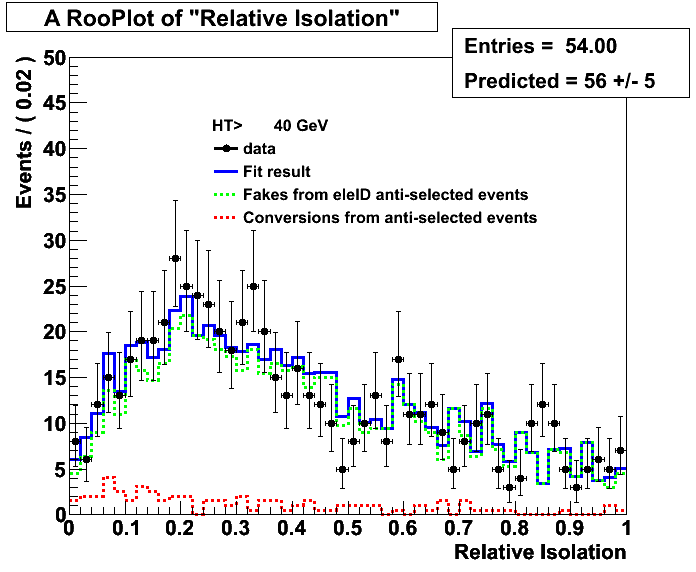
\includegraphics[scale=0.28]{Plots/caloIso_pt5_ht40.png}
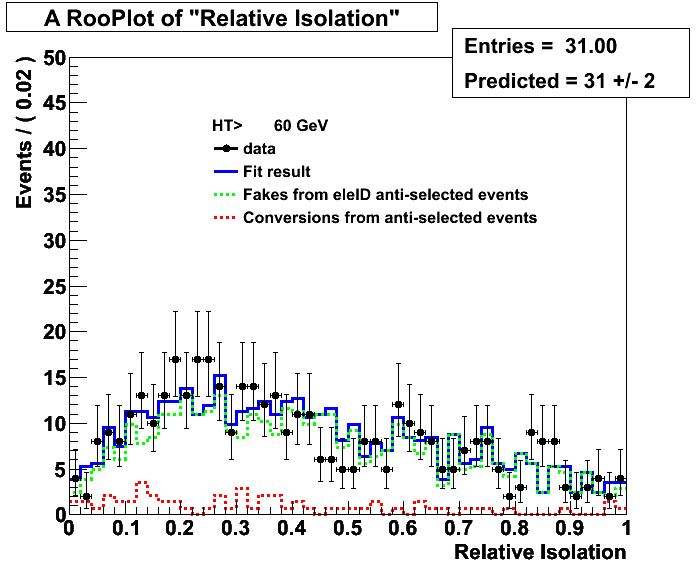
\includegraphics[scale=0.28]{Plots/caloIso_pt5_ht60.png}
\caption{Same as Figure~\ref{fig:caloIso_fit_HT} only this time for electrons with $P_T(e)>5$ GeV, always for the same three different values of the HT cut.}\label{fig:combIso_fit_HT_5}
\end{figure}

We summarize the result of the fits to the Calorimeter Isolation distribution in Table~\ref{tab:IsoFits}.  

\begin{table}[h!]
\vspace{5mm}
\begin{center}
\begin{tabular}{|c||c||c|c||c|c|}
\hline
& & Observed & Predicted & Observed &  Predicted \\
\hline
\hline
$H_{T}>20 \text{GeV}$ & CaloIso$<0.1$ & $115.$ & $115.4 \pm 7.5$ & $98.$ & $99.6 \pm 7.4$ \\
$H_{T}>40 \text{GeV}$ & CaloIso$<0.1$ & $54.$ & $56.5 \pm 5.3$ & $46.$ & $48.9 \pm 5.0$ \\
$H_{T}>60 \text{GeV}$ & CaloIso$<0.1$ & $31.$ & $31.8 \pm 2.6$ & $24.$ & $25.6 \pm 2.4$ \\
\hline
\end{tabular}
\end{center}
\caption{\textit{Summary of fit results predicting the number of electron that fall in the calorimeter Isolation region ($<0.1$), using the two-template fit. The data sample is taken from the SD JetMETTau of the 7TeV collision data, using the HLT\_Jet15U. }}
\label{tab:IsoFits}
\end{table}
\vspace{5mm}

%GEORGIA, can you please make this table...  [Summary of Number of events in the plots] from the six fits...

\subsection{Predicting the distribution of the $\alpha{_T}$ kinematic variable by inverting Electron ID Cuts}

Following the promising results of the $\alpha_{T}$ jet-balancing method previously described for the all-hadronic SUSY searches, it is a natural progression to look for extensions of this approach to the single-electron search, where a significant presence of QCD multi-jet backgrounds is expected.

The $\alpha_{T}$ variable is here defined as an N-object system where the set of objects is 1 electron and N-1 jets. This definition reproduces the kinematics of a di-jet system by contructing two pseudo-jets, which balance one another in $H_{T}$. The two pseudo-jets are formed from the combination of the N objects that minimizes the $\Delta H_{T} \equiv |H_{T,1} - H_{T,2}|$ of the pseudo-jets, and the resulting  $\alpha_{T}$ is
\begin{equation}
\alpha_{T} = \frac{1}{2} \frac{H_{T} - \Delta H_{T}}{M_{T}} =  \frac{1}{2} \frac{H_{T} - \Delta H_{T}}{\sqrt{H_{T}^{2}-MH_{T}^{2}}}.
\end{equation}

This section is dedicated to a first approach of commissioning the alphaT observable and study its behavior in pure fake electron events. It is therefore desirable to collect a suitable control sample which will be dominated by fake electrons and eliminate sources of prompt electron events (like W events).

One way to obtain such a sample is using the anti-selection method on electron ID variables which are less correlated with the missing transverse energy. In this section, we investigate the possibility of inverting the $\Delta \eta$(trk-SC) and $\Delta \phi$ (trk-SC) id cuts in the electron selection. The selected events in this method pass the pre-selection described in Section~\ref{sec:Sel}, while the anti-selected are those events which pass the selection with an electron that passes all selection id criteria except the $\Delta \phi$ (trk-SC) and $\Delta \eta$(trk-SC) ones. 

In order to establish the validity of the control sample obtained by the anti-selection method above, the perfomance must be compared of the leptonic $\alpha_T$ as obtained from the control sample and the actual QCD events passing the electron criteria defined in the ``signal'' region. As mentioned previously, SUSY events are expected to have high $H_{T}$, therefore it is essential to understand how the method evolves with increasing $H_{T}$ cuts. The number of events for 1pb$^{-1}$ passing the pre-selection, and two different cuts in $H_{T}$ are shown for selected in Table \ref{tab:CF_S_20} and for anti-selected in Table \ref{tab:CF_AS_20}. 

\begin{table}[h!]
\begin{center}
\begin{tabular}{|c||c|c|c|c|}
\hline
Cutflow & QCD EM enriched & QCD BC$\rightarrow e$ & QCDJets Pythia $\hat{p_{T}}$ &  W \\
\hline
\hline
All events & 5351938 & 256514.4 & 25470 & 17830 \\
N($e^{-}$) $\geq$ 1 & 15535.48 & 2529.63 & 2.26 & 2598.46\\
N($jets$) $\geq$ 1 & 10737.67 & 1668.66 & 2.26 & 666.30\\
HT $>$ 100 GeV & 661.13 & 69.95 & 2.26 & 68.98\\
HT $>$ 180 GeV & 79.73 & 7.52 & 2.18 & 16.10\\
\hline
\end{tabular}
\end{center}
\caption{\textit{Cutflow for both selected events.Numbers shown for 1pb$^{-1}$ for both QCD and W samples used for the anaylsis with electron $p_{T}$ requirement set to 20GeV.}}
\label{tab:CF_S_20}
\end{table}

\begin{table}[h!]
\begin{center}
\begin{tabular}{|c||c|c|c|c|}
\hline
Cutflow & QCD EM enriched & QCD BC$\rightarrow e$ & QCDJets Pythia $\hat{p_{T}}$ &  W \\
\hline
All events & 5351938 & 256514.4 & 25470 & 17830\\
N($e^{-}$) $\geq$ 1 & 29315.47 & 480.18 & 1.51 & 139.23 \\
N($jets$) $\geq$ 1 & 20452.26 & 325.28 & 1.51 & 33.32\\
HT $>$ 100 GeV & 942.99 & 17.21 & 1.51 & 2.91\\
HT $>$ 180 GeV & 79.74 & 1.64 & 1.43 & 0.66\\
\hline
\end{tabular}
\end{center}
\caption{\textit{Cutflow for anti-selected events.Numbers shown for 1pb$^{-1}$ for both QCD and W samples used for the anaylsis with electron $p_{T}$ requirement set to 20GeV.}}
\label{tab:CF_AS_20}
\end{table}

\subsubsection{Closure test with pure QCD background sample}

The control sample provided by anti-selection on the Delta ID Variables must first undergo a closure test with a pure QCD sample. This will show if there is any bias in QCD between the distribution of $\alpha_{T}$ in the selected and the anti-selected. The plots in \ref{fig:AlphaTbyHT} show the normalised shape of distributions, firstly before an $H_{T}$ cut (top left) and then as increasing cuts in $H_{T}$ are applied. The selected and anti-selected distributions show good agreement. The evolution of the $\alpha_{T}$ as $H_{T}$ cut increases shows the expected reduction in the tail for $\alpha_{T} >$ 0.55, the region of likely SUSY signal, for both selected and anti-selected.

\begin{figure}[h!]
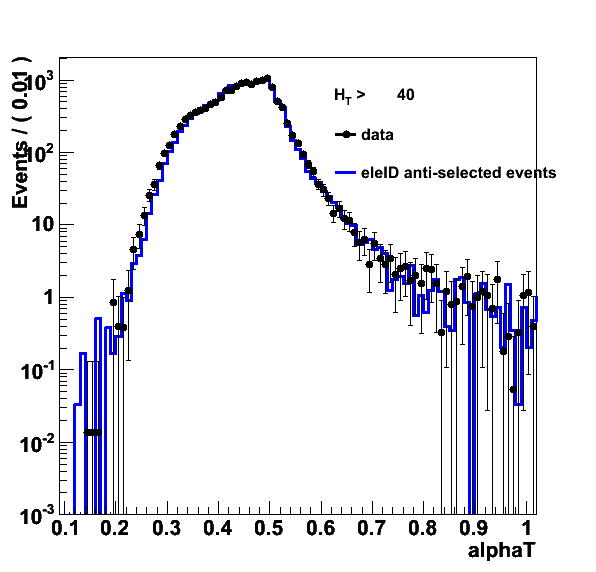
\includegraphics[width=50mm]{Plots/mc-alphaT-1}
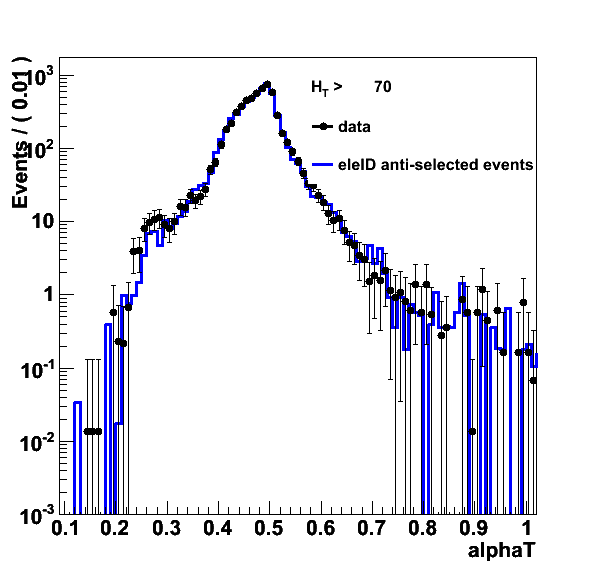
\includegraphics[width=50mm]{Plots/mc-alphaT-2}
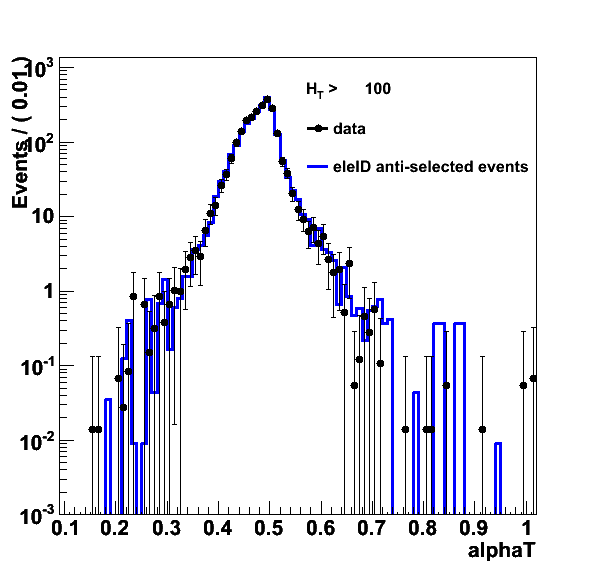
\includegraphics[width=50mm]{Plots/mc-alphaT-3}
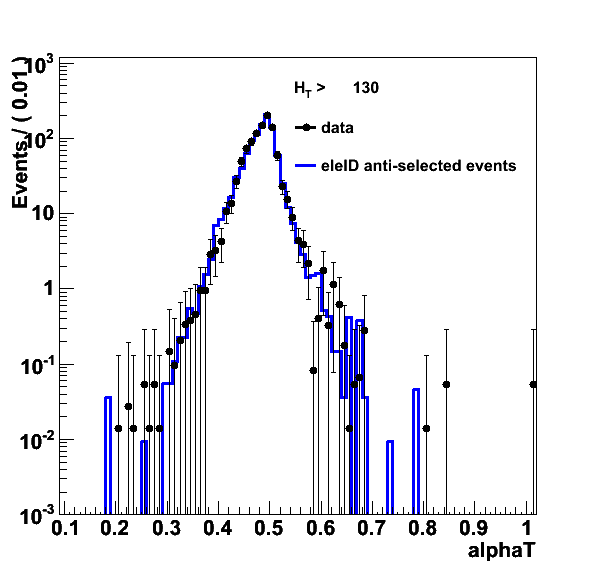
\includegraphics[width=50mm]{Plots/mc-alphaT-4}
\hspace*{3mm}
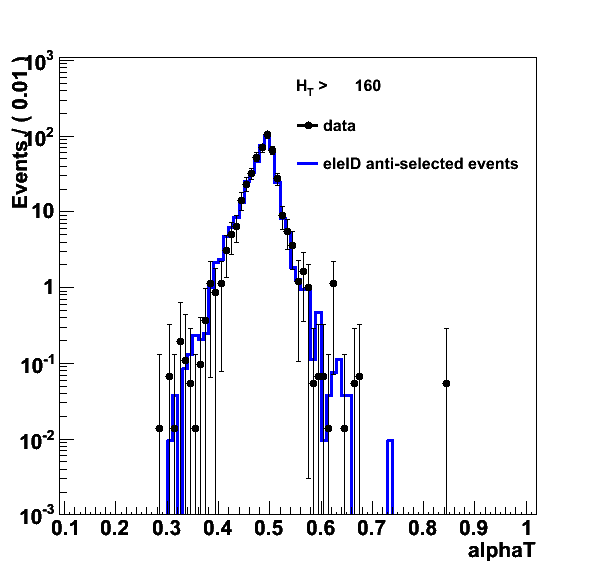
\includegraphics[width=50mm]{Plots/mc-alphaT-5}
\hspace*{3mm}
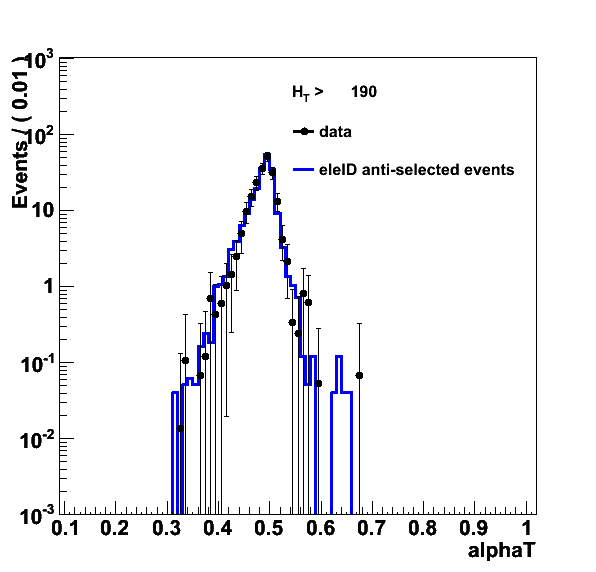
\includegraphics[width=50mm]{Plots/mc-alphaT-6}

\caption{\textit{The $\alpha_{T}$ distributions for selected (red) and anti-selected events (black) for the QCD multi-jet background, from inversion of the $\Delta \phi$ and $\Delta \eta$ ID Cuts, shown without HT cut (Top Left) and with progressive HT cuts (left-right, top-bottom). These distributions are normalised to unity for shape comparison. There is good agreement between the selected and anti-selected samples regardless of HT requirement, and the high $\alpha_{T}$ tails reduce as expected when moving to higher HT cuts.}}
\label{fig:AlphaTbyHT}
\end{figure}

In order to demonstrate the power of HT in $\alpha_{T}$ tail-reduction, we introduce the variable $R_{\alpha_T}$ which is defined as the ratio of the number of events passing the $\alpha_T$ cut over the number of events failing it:
\begin{equation}
R_{\alpha T} = \frac{N(\alpha_{T}>0.55)}{N(\alpha_{T}<0.55)}
\end{equation}
The ``default'' cut value here is the value prompted from the all-hadronic analysis, 0.55. Figure \ref{fig:AlphaT_Ratio} shows a plot of $R_{\alpha_T}$ as a function of the $H_{T}$ cut applied. As the $H_{T}$ requirement increases, $R_{\alpha_T}$ decreases in an exponential manner. Thic confirms that the noticable reduction in the tail are much more pronounced than those in the peak, therefore this is not a statistical effect only. The selected and anti-selected events remain in good agreement.

\begin{figure}[h!]
\begin{center}
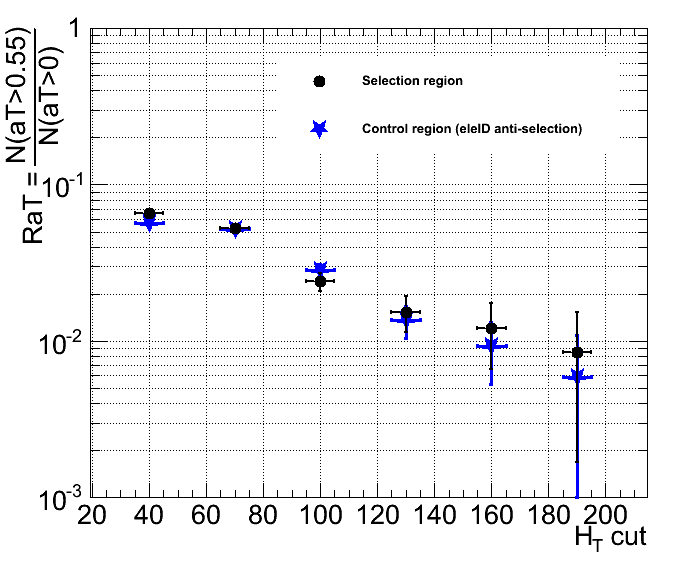
\includegraphics[width=100mm]{Plots/mc-alphaTratio}
\end{center}
\caption{\textit{The $R_{\alpha_T}$ versus the $H_{T}$ cut applied for the QCD multi-jet background, shown for both selected and anti-selected events in the Delta ID Inversion method.}}
\label{fig:AlphaT_Ratio}
\end{figure}

\subsubsection {Closure test with W + jets contamination in control region}

Having acertained the validity of the anti-selection method to predict the QCD contribution in the selected from the QCD in the anti-selected, it is important to test whether the process will work with contamination in the control region. The method is designed for data-driven extimation, and thus must be robust to such contamination.'

The closure test is repeated, with the anti-selected now from both the pure QCD sample as before, and W + jets also. The selected remains from pure QCD as a comparison. The normalised ditribution plots shown for this case are in Figure~\ref{fig:w-AlphaTbyHT}, and the plot of $R_{\alpha_T}$ as a function of the $H_{T}$ cut applied is in Figure~\ref{fig:w-AlphaT_Ratio}. 

\begin{figure}[h!]

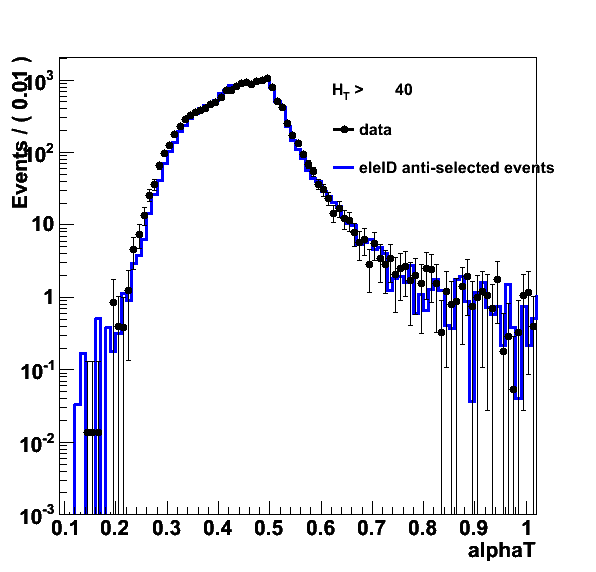
\includegraphics[width=50mm]{Plots/w-alphaT-1}
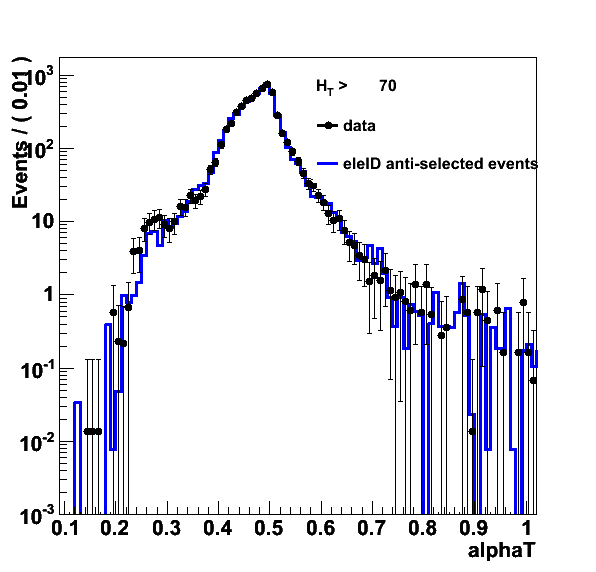
\includegraphics[width=50mm]{Plots/w-alphaT-2}
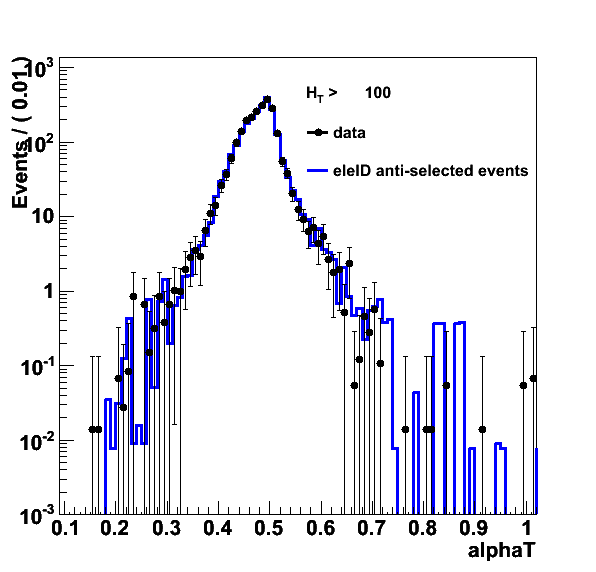
\includegraphics[width=50mm]{Plots/w-alphaT-3}
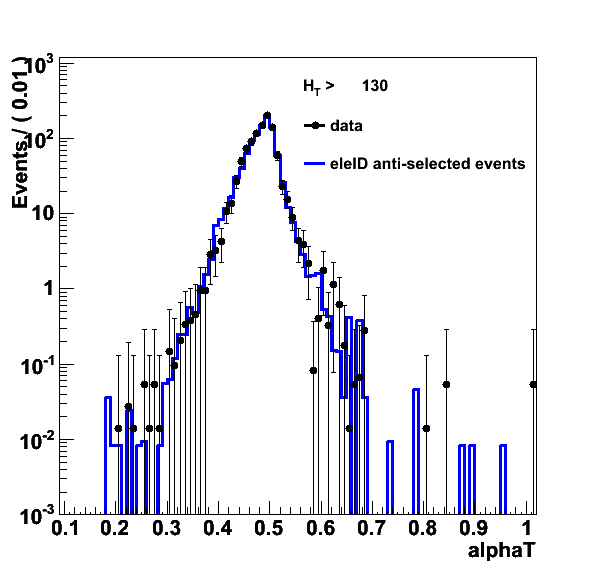
\includegraphics[width=50mm]{Plots/w-alphaT-4}
\hspace*{3mm}
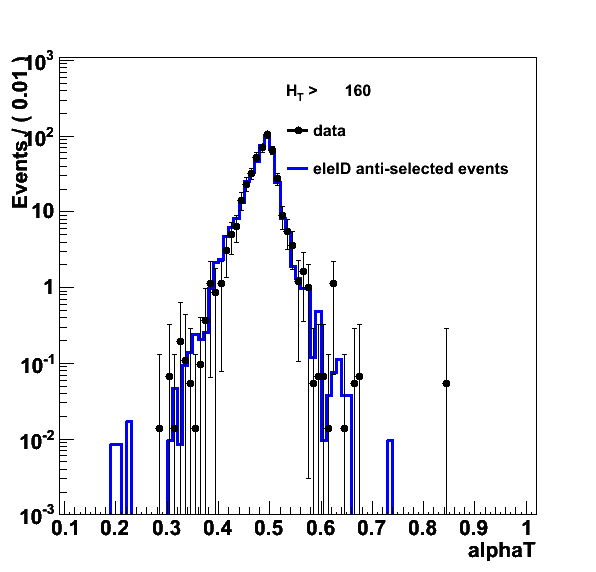
\includegraphics[width=50mm]{Plots/w-alphaT-5}
\hspace*{3mm}
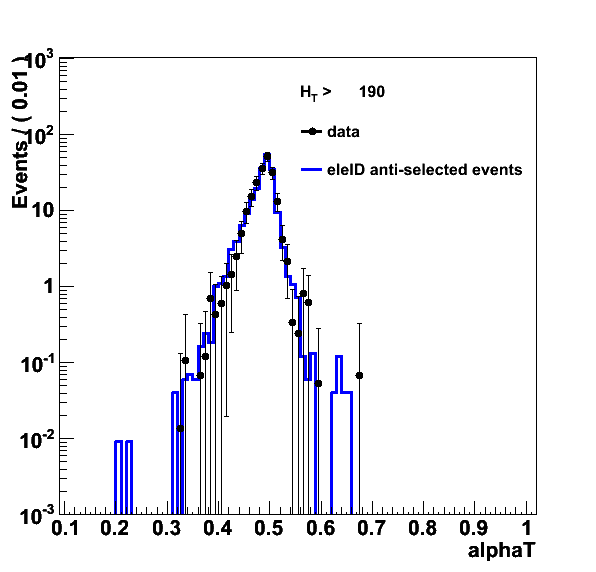
\includegraphics[width=50mm]{Plots/w-alphaT-6}
\caption{\textit{The $\alpha_{T}$ distributions for selected (red) and anti-selected events (black) for the QCD multi-jet background, and with signal contamination from W +jets in the anti-selected only, from inversion of the $\Delta \phi$ and $\Delta \eta$ ID Cuts, shown without HT cut (Top Left) and with progressive HT cuts (left-right, top-bottom). These distributions are normalised to unity for shape comparison. There is good agreement between the selected and anti-selected samples regardless of HT requirement, and the high $\alpha_{T}$ tails reduce as expected when moving to higher HT cuts.}}
\label{fig:w-AlphaTbyHT}
\end{figure}

 Figure \ref{fig:AlphaT_Ratio} shows a plot of $R_{\alpha_T}$ as a function of the $H_{T}$ cut applied. As the $H_{T}$ requirement increases, $R_{\alpha_T}$ decreases in an exponential manner. Thic confirms that the noticable reduction in the tail are much more pronounced than those in the peak, therefore this is not a statistical effect only. The selected and anti-selected events remain in good agreement.

\begin{figure}[h!]
\begin{center}
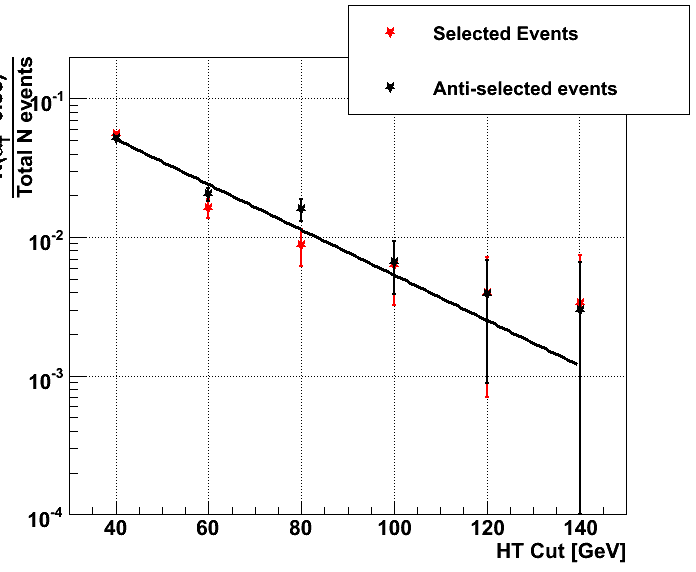
\includegraphics[width=100mm]{Plots/w-alphaTratio}
\end{center}
\caption{\textit{The $R_{\alpha_T}$ versus the $H_{T}$ cut applied for the QCD multi-jet background, with contamination from W + jets in the anti-selected only, shown for both selected and anti-selected events in the Delta ID Inversion method.}}
\label{fig:w-AlphaT_Ratio}
\end{figure}

Adding in contamination from the W + jets sample has no discernable effect on the shape of the $\alpha_{T}$ distribution, and the ratio remains to good agreement also. The control sample is thus robust to such a contamination, and still remains a good estimator of the shape of the QCD background for the selected events.

\subsubsection{Closure test with lowered electron $P_{T}$ threshold}
It is also important to commission $\alpha_{T}$ as the electron $p_{T}$ requirement is lowered. The study is repeated with the electron $p_{T} >$ 10 GeV. Tables \ref{tab:CF_S_10} and \ref{tab:CF_AS_10} show the numbers for selected and anti-selected cutflows respectively at $1pb^{-1}$. 

\begin{table}[h!]
\begin{center}
\begin{tabular}{|c||c|c|c|c|}
\hline
Cutflow & QCD EM enriched & QCD BC$\rightarrow e$ & QCDJets Pythia $\hat{p_{T}}$ &  W \\
\hline
All events & 5351938 & 256514.4 & 25470 & 17830 \\

N($e^{-}$) $\geq$ 1 & 22120.98 & 13117.37 & 4.37 & 2953.69\\

N($jets$) $\geq$ 1 & 14783.29 & 7811.25 & 4.37 & 761.22\\

HT $>$ 100 GeV & 846.64 & 312.95 & 4.37 & 78.73\\

HT $>$ 180 GeV & 159.83& 36.05 & 4.29 & 18.20\\
\hline
\end{tabular}
\end{center}
\caption{\textit{Cutflow for selected events.Numbers shown for 1pb$^{-1}$ for both QCD and W samples used for the anaylsis with electron $p_{T}$ requirement set to 10GeV.}}
\label{tab:CF_S_10}
\end{table}

\begin{table}[h!]
\begin{center}
\begin{tabular}{|c||c|c|c|c|}
\hline
Cutflow & QCD EM enriched & QCD BC$\rightarrow e$ & QCDJets Pythia $\hat{p_{T}}$ &  W \\
\hline
All events & 5351938 & 256514.4 & 25470 & 17830\\
N($e^{-}$) $\geq$ 1 & 44807.39 & 1406.28 & 3.30 & 173.04\\
N($jets$) $\geq$ 1 & 30089.89 & 920.40 & 3.30 & 43.52\\
HT $>$ 100 GeV & 1291.41 & 51.64 & 3.29 & 4.05\\
HT $>$ 180 GeV & 112.68 & 5.55 & 3.20 &  0.92\\
\hline
\end{tabular}
\end{center}
\caption{\textit{Cutflow for anti-selected events.Numbers shown for 1pb$^{-1}$ for both QCD and W samples used for the anaylsis with electron $p_{T}$ requirement set to 10GeV.}}
\label{tab:CF_AS_10}
\end{table}


\subsection{Isolation Templates}
